\section{Laplace transform}
\todo[inline, color=other]{The following section is essentially a complete rewrite of the previous Laplace transform. Everything shows up in basically the same order, but it's built on better code (imo).}
One very important tool when learning control theory is the Laplace transform.
It's mostly used to solve differential equations. We will explain how to do that, as well as some other important rules often used in control theory.
However, first we need to do some groundwork and build what will essentially be the scaffolding for the Laplace transform.
There are two major tools we will use to implement the Laplace transform: A DSL for Complex Numbers and a datatype representing mathematical expressions, aptly named \cmd{Expression}. 
We will also include \cmd{FunNumInst} from DSLsofMath\footnote{https://github.com/DSLsofMath/DSLsofMath/}, which allows us to write addition etc. between functions (in more technical language: it's a \cmd{Num} instance for functions).

The DSL we will use for Complex Numbers is an extension of the one developed in section \ref{sec:complex}. The actual implementation is not important, but if you want to read it, see listing \ref{code:complex}.

%\todo[inline, color=lessurgent]{Do we want module declaration?}
\begin{code}
module Laplace where
import ComplexNumbers
import FunNumInst 
\end{code}

\todo[inline]{Maybe more introduction?}
%\todo[inline]{Either say we have extended Complex or use Complex from TSS?}


\subsection{The Expression datatype}
Like in section \ref{sec:integrals}, we create a recursive datatype. We will not
state it in it's entirety here, but you can find it in \ref{sec:code}. What we
will do is show some parts of it and talk about how they fit together. 

First, we declare a new datatype, which we call \cmd{Expression}, which takes a parameter \cmd{a}. 
\begin{code}
data Expression a = ...
\end{code}
The parameter is the type of the expression: we will mostly use \cmd{Expression Complex}, which in essence is a syntactic representation of a function of a complex variable.
After that, we give some examples of how to construct \cmd{Expression}s,
separated by \cmd{|}. The two most important of these are \cmd{Const a} and
\cmd{Id}. These represent the constant function and the identity function,
respectively. \todo{Can we assume they know what id is?} For example, 
\begin{example}
  Create the constant $2+3i$ as an \cmd{Expression}. 
\end{example}
\begin{solution}
~  
\begin{code}
testExp1 :: Expression Complex 
testExp1 = Const (Complex (2, 3))
\end{code} 
\end{solution}

The next four are the four arithmetic operations for \cmd{Expression}, e.g. we can create an \cmd{Expression} by adding two other together. 
Instead of just naming them \cmd{+}, \cmd{*}, etc. they are instead named with
colons around them, e.g. \cmd{:+:}. This is in order to highlight that it is
addition between expressions.
% \todo[inline]{Explain the different parts - how they recurse, how to create new expressions.}
%\todo[inline]{Give example, compare to math}
\begin{example}
Now, you might wonder what an actual expression might look like. Well, look no further:

\begin{code}
testExpression :: Expression Complex
testExpression = Sin (Const 3 :*: Id) :+: Exp (Negate (Id))
\end{code}
  which in math can be written
\begin{equation*}
  f = \fcn{t}{\sin (3t) + e^{-t}}
\end{equation*}
\end{example}
One way to visualise \cmd{Expression}s is to drawn them in syntax tree, see
\ref{fig:expression-syntax-tree}. \todo{Explain what happens in the picture.}
\begin{figure}
  \centering
  \begin{tikzpicture}
    \node[above] {\cmd{:+:}};
    \draw (0,   0) -- (-1, -1) node[left]  {\cmd{Sin}};
    \draw (-1, -1) -- (-2, -2) node[left]  {\cmd{:*:}};
    \draw (-2, -2) -- (-3, -3) node[left]  {\cmd{Const 3}};
    \draw (-2, -2) -- (-1, -3) node[right] {\cmd{Id}};
    \draw (0 ,  0) -- (1 , -1) node[right] {\cmd{Exp}};
    \draw (1 , -1) -- (2 , -2) node[right] {\cmd{Negate}}; 
    \draw (2 , -2) -- (3 , -3) node[right] {\cmd{Id}}; 
  \end{tikzpicture}
  \caption{Sketch of a syntax tree; I imagine there being either small circle around each command or possibly just space (like in Communicating Mathematics ...)}
  \label{fig:expression-syntax-tree}
\end{figure}

\begin{exercise}
Create your own test expression.
\end{exercise}
%\todo[inline]{Explain eval, and how that takes a syntactic representation to a semantic one. }
Now, we've mentioned how \cmd{Expression} is a syntactic
representation of some sort of semantic expression. What does this mean and what
is the semantic expression? Well, the expressions we have written seem to
represent mathematical expressions alright, but we can't really do anything with
them. Besides, there are many mathematical properties we aren't really capturing
with \cmd{Expression} --- for example, \cmd{Const 1 :+: Const 2 == Const 2 :+:
  Const 1} is \cmd{False}, they aren't equal. Of course, we know that
mathematically $1+2=2+1$. How do we solve this disconnect between math and our DSL? 
We've previously mentioned \todo{Right?} that we'll distinguish between syntax and
semantics. So far, this section has discussed syntax a lot, but not really semantics. What
do our \cmd{Expression}s represent? That's where the semantics come in, they are
the meaning of our \cmd{Expression}s. To move from the syntactic level to the
semantic, we will define a function \cmd{eval} which takes us from the syntactic
level to the semantic one. 
We will then have to define the semantics somehow so that this is actually the case. 
The full function is quite long and works through pattern matching. \todo{Do we
  want to list it or just take parts of it now, letting the entirety of it be
  found in the appendix?}
\begin{code}
shift :: Num a => a -> (a -> a) -> (a -> a)
shift tau f = \t -> f (t-tau)

eval :: (Num a, Floating a, Eq a) => Expression a -> a -> a
eval (Const c)           = \t -> c
eval Id                  = id
eval Pi                  = eval (Const pi)
eval (e1 :+: e2)         = eval e1 + eval e2
eval (e1 :*: e2)         = eval e1 * eval e2
eval (Shift tau e)       = \t -> (shift tau) (eval e) t -- shifts e by tau, i.e. begins after tau seconds
eval (Negate e)          = negate (eval e)
eval (Exp e)             = exp    (eval e)
eval (Sin e)             = sin    (eval e)
eval (Cos e)             = cos    (eval e)
eval (Tan e)             = tan    (eval e)
eval (Asin e)            = asin   (eval e)
eval (Acos e)            = acos   (eval e)
eval (Atan e)            = atan   (eval e)
eval (Integral   e e0)   = undefined -- TODO
eval (Derivative e e0)   = undefined -- TODO
\end{code}
\begin{figure}
  \centering
  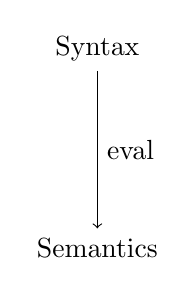
\begin{tikzpicture}
    \node[above] {Syntax};
    \draw     (0, 0)  -- (0, -1) node[right] {\cmd{eval}};
    \draw[->] (0, -1) -- (0, -2) node[below] {Semantics};
  \end{tikzpicture}
  \caption[Diagram: syntax, eval, semantics]{Diagram showing the syntactic and
    semantic levels, as well as the eval function between them. (The arrowhead
    is a little small)}
  \label{fig:diagram-eval}
\end{figure}
%\todo[inline]{Exercise: create an expression, run eval on it?}
\begin{example}
  Run \cmd{eval} on \cmd{testExpression} above, insert some values and compare
  to the mathematical function. 
\end{example}
\begin{solution}
  The expression
\begin{code}
 -- TODO
tmp = eval testExpression
 -- testExpression = Sin (Const 3 :*: Id) :+: Exp (Negate (Id))
\end{code}
  \todo[inline]{finish solution}
\end{solution}
\begin{exercise}
  Create your own expression and run the eval function on it. Make sure to test
  some values, ensuring that the semantic function gives the right values.
  \todo[inline]{I'm thinking that either they download the code themselves, or if
    they're on website they run it on the site.}
\end{exercise}
\todo[inline]{Write something about the types?}

\subsubsection{Some conventions and notations}
Sometimes in math books there is some notational abuse: does $f(t)$ mean the
function $f$ or $f$ applied to the value $t$? Often times we can understand
which is meant from context, but not always. We will avoid this problem by being
explicit when a function is applied to a value or not: the function will be written
$f$, the function applied to a value will be written $f(t)$. Sometimes we need
to write out the functions definition explicitly. If so, we will write it out
using $\fcn{}{}$: for example, writing that $f$ is the exponential function will
be $f = \fcn{t}{e^{t}}$.

Another convention we will use is that when talking about a function named with
a letter, for example $f$, we will sometimes denote the Laplace transform of
said function with the capital version of the letter, e.g. $F$. Put more
succinctly: $F$ is the Laplace transform of $f$. This could be confused for the
primitive function of $f$, but we will be explicit whenever we talk about
primitvie functions instead of Laplace transforms. We know, we haven't even spoken
about the Laplace transform yet, but keep it in mind for the following sections.
One notation we won't use but which might show up in other literature
is to write $\tilde{f}$ for the Laplace transform of $f$. 
% \todo[inline]{Will refer to functions without parameter if possible, use lambda calc if not. f(t) means f applied to t.}
% \todo[inline]{L (f) = F, unless stated otherwise. $\tilde{f}$ sometimes used, we shant. We use {} instead of (); some others do, some dont'. Disambiguate.}
\subsection{The definition and corresponding types}
Before we start: this section will start a little bit math heavy. Don't be
discouraged. We will give the mathematical definition of the Laplace transform,
take it apart a little and analyse the types. When we're done with that,
however, we will just skip the calculating and show some shortcuts. If you're
feeling like the math just isn't making sense, you can safely jump to section
\ref{sec:common-rules}. 

Now, no more skirting around the issue, here's the definition of the Laplace
transform $\Lplc$: 
\begin{equation*}
 \Lplc \{f\} = \fcn{s}{\int_0^\infty e^{-st}f(t) \dd t}. 
\end{equation*}
\todo{Technically, we aren't following our own rules: we should've written
  $\Lplc = \fcn{f,s}{\int_0^\infty ... \dd t}$. Do we want to do this? }
There's a lot going on here. On the left hand side we have two symbols: $\Lplc$
and $f$. We see that $f$ shows up on the other side of the equation, meaning
it's bound over the equality. On the right hand side, there are a few things to
see: we have an integral from $0$ to infinity, we have the function $f$ again,
and we have an exponential function. Note that due to $t$ being bound by the
integral, the exponential is a function of $s$ in the wider scope. 
Thus the Laplace transform of a function $f$ is an integral of that function
multiplied by an exponential function.

One way to write it could be: 
\begin{code}
laplace' :: Expression Complex -> Expression Complex -> Expression Complex
laplace' f e = Integ (Const 0) (Infinity) (exp :*: f) 
               where exp = Exp (Negate (e) :*: Id) 
-- TODO: Does not compile currently due to Infinity. Maybe say it's pseudocode? 
\end{code}

\todo[inline]{Look at the types of all the parts, write some more on it.}


% \todo[inline]{If the math scares you, don't be discouraged. We will show you shortcuts later.}
% \todo[inline]{State definition.}
%\todo[inline]{Write in Expression form}
However, this is really annoying to calculate. Besides, writing a proper
definition of how to evaluate \cmd{DefInteg} is really, \emph{really} hard. We
don't want to do to that. Instead, what we will do is to show you how to use a
table to calculate transforms. 
% \todo[inline]{This is garbage to actually calculate.}
% \todo[inline]{We will use rules instead.}

Some conventions we will use that are not strictly related to the Laplace
transform is that we will write addition and multiplication between (real and complex) numbers
the same way as we do between (real and complex) functions, using the ordinary
symbols $+$ and $\cdot$, i.e. we will treat them as polymorphic types. 
We will however be consistent and write out $\cdot$ instead of just keeping to
functions next to each other (e.g. $x \cdot y$ instead of $xy$).
% \todo[inline]{Maybe mention $+$ and $\cdot$ between reals and between functions.}
\subsection{Common rules, how to use them}\label{sec:common-rules}
\todo[inline]{Add recreation of the table they're allowed to use during exam, maybe?}

\begin{table}
    \centering
    \caption{Two tables of the Laplace transform.}
    \label{fig:laplace_tables}
\begin{subfigure}{0.999\textwidth}
    \centering
    \caption{Laplace transform ordinary}
    \label{fig:laplace_table_ord}
    \begin{tabular}{c|c}
    $f$ & $F$ \\
    $\fcn{t}{y(t - T)}$ & $\fcn{s}{e^{-sT}Y(s)}$
    \end{tabular}
\end{subfigure} \\
\begin{subfigure}{0.999\textwidth} 
    \centering
    \caption{Laplace transform in code; see \ref{code:laplace-def} for full definition}
    \label{fig:laplace_table_code}
    \begin{code'}
-- rules
laplace :: Expression Complex -> Expression Complex -- TODO: maybe instead do Time->Freq
laplace (e1 :+: e2) = laplace e1 :+: laplace e2 -- Superposition
laplace (Const a :*: e) = Const a :*: laplace e -- scaling
laplace (Derivative e e0) = Id :*: laplace e :-: (Const e0) -- L {f'} = \s -> s * L {f} - f(0)
laplace (Integral e e0) = laplace e :/: Id -- L {int_0^t f(x) dx} = s -> L {f} /s 
laplace (Shift tau e) = Exp (Id :*: Const tau) :*: laplace e -- TODO: double check signs
  -- TODO: double check signs on next two
laplace (Exp (Negate (Const tau :*: Id)) :*: e) = Shift tau (laplace e)
laplace (Conv e1 e2) = laplace e1 :*: laplace e2 -- convolution turns into multiplication
-- transforms
laplace (Impulse) = Const 1 -- L {delta(t)} = \s -> 1
laplace (Const 1) = Const 1 :/: Id -- L {a} = \s -> a/s; a = 1 => L {1} = 1/s
laplace (Id)      = Const 1 :/: (Id :*: Id) -- L {t} = \s -> 1/(s^2)
laplace (Exp (Negate (Const a :*: Id))) = Shift (negate a) (Const 1 :/: Id)-- TODO: Check signs
laplace (Const 1 :-: Exp (Negate (Const a :*: Id))) = Const a :/: (Id :*: Shift a Id) -- TODO: Doublecheck signs. Also, is this necessary?

laplace (Exp (Negate (Const a)) :-: Exp (Negate (Const b))) = Const (b - a) :/: (Shift (negate a) Id :*: Shift (negate b) Id)
laplace (Id :-: (Const 1 :-: Exp (Negate (Const a) :*: Id)) :/: Const a) = Const a  :/: (Id :*: Id :*: Shift (negate a) Id)
laplace (Const 1 :-: (Const 1 :+: Const a :*: Id) :*: Exp (Negate (Const a) :*: Id)) = Const (a*a) / (Id :*: Shift (Negate a) (Id :*: Id)) -- Const a :*: Const a instead of Const (a*a)?
-- TODO: Doublecheck signs on the next two
laplace (Exp (Negate (Const a :*: Id)) :*: Sin (Const omega :*: Id)) = Const omega :/: (Shift a (Id :*: Id) :+: (Const (omega*omega)))
laplace (Exp (Negate (Const a :*: Id)) :*: Cos (Const omega :*: Id)) = (Shift a Id) :/: (Shift a (Id :*: Id) :+: (Const (omega*omega)))
    \end{code'}
\end{subfigure}
\end{table}
Throughout this section we will show you how to use the rules in the table to
calculate Laplace transforms, since that makes life a lot easier. 

The Laplace
transform $\Lplc$ will be implemented as the command \cmd{laplace}, e.g.
\cmd{laplace e} is the Laplace transform of the expression \cmd{e}.
See \cmd{laplace} below for the table adapted to our DSL. Note: this is not the
full implementation, it's just a refrasing of the table. For the full
implementation, see appendix (Listing
\ref{code:laplace-def})\todo{Make sure this is correct with correct reference.}

Before we
start, one important property: if two
functions have the same Laplace transform, then they are the same function. In
our DSL this means that \cmd{eval (laplace e)}
\todo[inline]{Note: I'm not certain the Shift:s are correct or whether there should be a
  negate there somewhere, thus I've done TODO:s on all I'm not sure get the
  correct sign. Also, this is still in development, needs cleanup.}

\subsubsection{Superposition}
One of the most important rules of the Laplace transform is what's often called
either superposition or linearity. Informally (and a little imprecisely), it means that we know the
Laplace transfers of two functions, the Laplace transform of their sum is the
sum of the Laplace transforms. Mathematically, it's often phrased
\begin{equation*}
 \Lplc \{\alpha f + \beta g\} = \alpha \Lplc \{f\} + \beta \Lplc \{g\}.
\end{equation*}
Thus, if we know that the Laplace transforms of $f$ and $g$ are $F$ and $G$,
respectively, then the Laplace transform of $f + g$ would be $F + G$.

Superposition is a rule which might on first glance seem like it doesn't say
anything. However, it's also often used by students without them knowing.
If we'd want to calculate $\Lplc\{\fcn{t}{e^{t} + e^{-t}}\}$, for example,
knowing that 
\begin{equation*}
  \Lplc\{\fcn{t}{e^{t}}\}  = \fcn{s}{\frac{1}{s-1}}
  \end{equation*}
and that 
  \begin{equation*}
  \Lplc\{\fcn{t}{e^{-t}}\} = \fcn{s}{\frac{1}{s+1}}
\end{equation*}
does not help us anything if we don't have superposition.
Of course, we do have superposition, so we know that
\begin{align*}
  \Lplc\{\fcn{t}{e^{t}+e^{-t}}\} &= \Lplc\{ \fcn{t}{e^t} \} + \Lplc\{\fcn{t}{e^{-t}}\} \\
                                &= \fcn{s}{\frac{1}{s-1}   + \frac{1}{s+1}}.
\end{align*}
transforms. 
Thus superposition is one of our most useful tools when calculating Laplace
transforms. 

But how about calculating Laplace transforms of \cmd{Expressions}? 
Luckily, superposition is fairly easy to implement in our DSL, so we can use the
same rules to calculate transforms of \cmd{Expression}s!
We get the following snippet: 
\begin{code}
laplace (e1 :+: e2) = laplace e1 :+: laplace e2 
\end{code}
i.e. the Laplace transform of a sum of \cmd{Expression}s is a sum of
\cmd{Expression}s that are the result of applying \cmd{laplace}, just as we
wanted. \todo{This is some sort of morphism, right? Mention this in a footnote, for the category
  theoretic-minded student?}
Note that we have \cmd{:+:} between both the expressions \cmd{e1} and \cmd{e2}
and their respective Laplace transforms, since they are all of type
\cmd{Expression}. Had \cmd{laplace} not returned an \cmd{Expression}, we might
need to define a new addition. 


%\todo[inline]{Most basic rule, otherwise would be very annoying. Give example of "even knowing F and G would not let us calculate L {f+g}."}
%\todo[inline]{Show implementation}
%\todo[inline]{Discuss types}
\subsubsection{Derivative rule}
Another very important rule regards the Laplace transform of a derivative. This
is important because it helps us solve (some) differential equations a lot
easier. It's also used to more easily implement and calculate PID controllers.

Informally, the rule can be described as turning differentiation into
multiplication (and subtraction of an initial value). 
Mathematically, this can be written
\begin{equation*}
  %\Lplc\left\{\fcn{t}{\dv{t} f(t)}\right\} = \fcn{s}{s \cdot \Lplc\{f\}(s) - f(0)}
  \Lplc\left\{\fcn{t}{f'(t)}\right\} = \fcn{s}{s \cdot \Lplc\{f\}(s) - f(0)}
\end{equation*}
i.e. if we have a derivative of a function, the corresponding Laplace transform
is the Laplace transform of the function (not the derivative) multiplied with
id. Finally we subtract the function evaluated in 0. It's not uncommon for $f(0)
= 0$, which makes the rule even easier. 
 
In our DSL, the rule is represented:
\begin{code}
laplace (Derivative e e0) = Id :*: laplace e :-: (Const e0) 
\end{code}
% kommentar i koden: -- L {f'} = \s -> s * L {f} - f(0)
i.e. the derivative of \cmd{e} with inital value \cmd{e0} has Laplace transform \cmd{Id} multiplied
with the Laplace transform of \cmd{e} minus the constant \cmd{Const e0}.

\begin{example}
  Solve the differential equation
  \begin{equation*}
   f = -f' \qc f(0) = 1
 \end{equation*}
 by applying the Laplace transform on both sides of the equation and setting
 them equal.
\end{example}
\begin{solution}
~
  \todo[inline]{I just noticed a mistake I made early, so there are likely sign errors
    throughout this example. TODO: Make sure it's correct. }
Unfortunately, we can't just ask our DSL to solve the equation - it isn't
advanced enough. However, we can use some pseudocode to reason about it.
%To avoid the problem of functions which are semantically the same but
%syntactically different, we will include \cmd{eval} in our reasoning.
Remember that if two functions have the same Laplace transform they are equal.
In our case, this means that if we can find a function such that
\cmd{laplace e == laplace (Derivative e 1)}, then we know that \cmd{e} is a
solution to the diffential equation. 
\begin{code}
  laplace (Derivative e 1)
== {- derivative rule -}
  Id :*: laplace e :-: Const 1
== {- from differential equation -}
  laplace e
\end{code} 
So far so good. We've shown that for \cmd{e} to be a solution to the
differential equation, we also need it to satisfy the equation \cmd{laplace e ==
Id :*: laplace e :-: Const 1}, which translated into mathematics means
$\Lplc\{f\} = \fcn{s}{s F(s) - 1}$.

Now you might think ``We've exchanged one
equation for another, how does that help us?'', which is a valid question. So
what is the rationale for this? Well, when given the choice to solve one of the
two following equations
\begin{align*}
  f &= f' \qc f(0) = 1 \\
  F &= \fcn{s}{s F(s) + 1}
\end{align*}
we know which one we'd prefer.

Hint: it's the second.

The first is a differential equation, which 
requires great guesswork or some more advanced methods to solve, while the second one is
solvable using simple algebra.
Solving the second equation results in the function $F =
\fcn{s}{\frac{1}{s-1}}$. Looking at your favorite table of Laplace transforms,
you might find somewhere the formula $\Lplc\{\fcn{t}{e^{-at}}\} =
\fcn{s}{\frac{1}{s+a}}$ (or \cmd{laplace (Exp (Const a :*: Id)) = Const 1 :/:} \cmd{(Id - Negate (Const a))},
 and if that's the case, we're flattered that's your
  favorite table of transforms!) \todo{Make sure it's the correct formula} If we
  let $a = 1$, we see that this is the function we found!
  Thus we can conclude that the function we're looking for is
  $\fcn{t}{e^{-t}}$.

Now, we're technically done. However, a good idea when solving differential
equations (using the Laplace transform or another method) is to check whether
the found solution actually satisfies the equation.

Typically this means two things: differentiating the found function (maybe
several times, depending on the order of the equation), and then inserting the
result in one side of the equation, seeing if it's possible to get to the other.

In our case, this means differentiating $\fcn{t}{e^{-t}}$. From single variable
calculus (or Beta) we get
\begin{equation*}
 \fcn{t}{\dv{t} f(t)} =  \fcn{t}{\dv{t}e^{-t}}= \fcn{t}{-e^{-t}} = -f,
\end{equation*}
i.e. the function satisfies the equation.

Now we just need to check the initial value:
\begin{equation*}
  f(0) = e^{-0} = 1,
\end{equation*}
which is what we wanted, and thus we're done.
\end{solution}

%\begin{code}
%diffeq :: Expression Complex -> Expression Complex 
%diffeq e = e :+: (Derivative e 1)
%\end{code}
% \todo[inline]{Allows us to solve diff eqs.}
% \todo[inline]{Also used in PID}
%\todo[inline]{Show rule}
\todo[inline]{Discuss types}
\subsubsection{Integral rule}
Just like we can use the Laplace transform to transform differentiation into
multiplication, we can use it to transform integration into division. This is
also used for PID controllers.

Mathematically, the rule is
\begin{equation*}
 \Lplc \left\{\fcn{t}{\int_0^t \fcn{x}{f(x)} \dd x}\right\}  = \fcn{s}{\frac{\Lplc\{f\}}{s}}.
\end{equation*}
Note that the integral is a function of $t$. 
\todo{I'm not sure about the $\fcn{x}{f(x)}$ in the integral.}

In our DSL, this is written:
\begin{code}
laplace (Integral e e0) = laplace e :/: Id 
\end{code}

%\todo[inline]{Is used for PID}
%\todo[inline]{Show rule}
\todo[inline]{Discuss types}
\subsubsection{Convolution}\label{sec:convol}
The convolution of two functions $f$ and $g$ is written $f \conv g$, defined
\begin{equation*}
f \conv g = \int_0^t f(\tau) g(t-\tau) \, \dd\tau.
\end{equation*}
\todo[inline]{Types!}
Convolution is used in many applications, but the one that's likely most
important is when looking at a system. 

\begin{figure}[H]
\centering
\begin{tikzpicture}[auto, node distance=2cm,>=latex']
    % Placing the blocks
    \node [input, name=input] {};
    \node [block, right of=input] (g) {G(s) / g(t)};
    \node [block, right of=g,
            node distance=3cm] (h) {H(s) / h(t)};
    % Arrows 1 
    \draw [->] (g) -- node[name=u] {k} (h);
    \node [output, right of=h] (output) {};

    % Arrows 2
    \draw [draw,->] (input) -- node {u} (g);
    \draw [->] (h) -- node [name=y] {y}(output);
\end{tikzpicture}
\caption{A simple block diagram showing a subsystem with transfer function G(s)
  feeding into a subsystem with transfer function H(s). u(t) and y(t) are the
  in- and output signals, respectively. k(t) is the input of the H-system and
  output of the G-system. Adapted from \ref{fig:tfex}}
\label{fig:conv-system}
\end{figure}

\todo{Fill this (incomplete) description out.}

Typically, what we want to do is Laplace transform this expression, as that
turns convolution into multiplication.

Mathematically, this means
\begin{equation*}
 \Lplc\{f \conv g\} = \Lplc\{f\} \cdot \Lplc \{g\} = F \cdot G
\end{equation*}
and in our DSL, this is written
\begin{code}
laplace (Conv e1 e2) = laplace e1 :*: laplace e2
\end{code}

This turns the expression above into
\todo{Fill this out}

%\todo[inline]{Explain Convolution}
%\todo[inline]{Explain usage}
%\todo[inline]{Show rule}
\todo[inline]{Discuss types}
\subsubsection{Time shift}
The time shift rule allows us to start a system later, i.e. 
\todo[inline]{Used when we want a system to start later}
\todo[inline]{Show rule}
\todo[inline]{Discuss types}
\subsubsection{Exponential decay (frequency shift)}\label{sec:decay}
\todo[inline]{Used to "dämpa" a system.}
\todo[inline]{Can be seen as frequency shift, i.e. analog to timeshift. Mention homomorfism?}
\todo[inline]{Show rule}
\todo[inline]{Discuss types}
\subsection{Inverse laplace transform}

So far, whenever we've found an expression for the Laplace transform of a function, we've handwaved it by saying ``and we recognize that this other function transforms into this function, thus it should be the answer''. This gives the right answer (obviously, or else we wouldn't teach you that...), but it's not entirely rigorous (and mathematicians love rigor!)

The ``proper'' way to do it is by using what's (appropriately) called the inverse Laplace transform.
% The reason we've done this is because... 

Like the regular Laplace transform, the inverse Laplace transform is defined using an integral. This one is even more clunky than the ordinary Laplace transform, however. The definition goes that the inverse Laplace transform of a function $F$, denoted $\Lplc^{-1}\{F\}$,  is given by

\begin{equation*}
    \Lplc^{-1} \left\{F\right\} s = \frac{1}{2\pi} \lim_{T\to\infty} \int_{\gamma - iT}^{\gamma + iT} e^{st} F(s) \dd s.
\end{equation*}

Now, your reaction here might be: what's this monstrosity? An integral where both endpoints are complex numbers, and a limit outside of that? Luckily, we don't have to calculate it\footnote{However, if you want to understand how to calculate it, we recommend ``A First Course in Complex Analysis'', which is freely available at \url{http://math.sfsu.edu/beck/complex.html}}, since we can just use the rules to find the inverse instead! 



